\section{Scientific/Technical Methodology and Work Plan}\label{sec:methodology}
\begin{todo}{from the proposal template}
  A detailed work plan should be presented, broken down into work packages\footnote{A work
    package is a major sub-division of the proposed project with a verifiable end-point –
    normally a deliverable or an important milestone in the overall project.} (WPs) which
  should follow the logical phases of the implementation of the project, and include
  consortium management and assessment of progress and results. (Note that your overall
  approach to management will be described later, in Section 2).

Notes: The number of work packages used must be appropriate to the complexity of the work
and the overall value of the proposed project. The planning should be sufficiently
detailed to justify the proposed effort and allow progress monitoring by the Commission.

Any significant risks should be identified, and contingency plans described
\end{todo}
\newpage\subsection*{Overall structure of the work plan}

Our work plan is divided into seven scientific work packages.  The
first group of work packages is dedicated to the networking activities
that are needed to gather the proofs today located in different
libraries.  The second to making these proofs accessible, beyond
trans-national and virtual access.  The third to joint research
activities that prepare the future of Logipedia.

Together with these seven scientific work packages, two more work
packages are dedicated to dissemination, communication and
exploitation and to management.

\begin{longtable}{|p{0.05\textwidth}|p{0.15\textwidth}|p{0.17\textwidth}|p{0.55\textwidth}|}
\hline
\rowcolor{color2}\multicolumn{4}{|l|}{\bf Networking activities:}\\
\hline
WP1
&
Integration &
Jesper Cockx

(Delft)
&
Instrument the systems for which we already know how to encode the
proofs in Dedukti, and make these proofs available in Logipedia.
\\
\hline
WP2
&
Automatic theorem proving
&
Chantal Keller

(Saclay)
& 
Develop automatic theorem provers to populate,
help, and benefit from Logipedia.
\\
\hline
WP3
&
Large libraries
&
Tobias Nipkow

(M\"unchen)
&
Export large dedicated libraries in curated form 
to Logipedia for end-user applications.
\\
\hline
\end{longtable}

\begin{longtable}{|p{0.05\textwidth}|p{0.15\textwidth}|p{0.17\textwidth}|p{0.55\textwidth}|}
\hline
\rowcolor{color2}\multicolumn{4}{|l|}{\bf Trans-national and virtual access:}\\
\hline
WP4
&
Access
&
Frédéric Blanqui

(Inria)
&
Define and build the Logipedia hardware and software infrastructure in
which the proofs will be integrated.
\\
\hline
WP5
&
Structure of the encyclopedia
&
Florian Rabe

(Erlangen)
&
Provide infrastructure for the structured ontological representation
of libraries and use it to enrich the information about formal
libraries in Logipedia.
\\
\hline
\end{longtable}


\begin{longtable}{|p{0.05\textwidth}|p{0.15\textwidth}|p{0.17\textwidth}|p{0.55\textwidth}|}
\hline
\rowcolor{color2}\multicolumn{4}{|l|}{\bf Joint research activities:}\\
\hline
WP6
&
Theories
&
Cezary Kaliszyk

(Inssbruck)
&
Bringing proof systems implementing a theory 
that has not yet been expressed in Dedukti to LIL 2 or better.
\\
\hline
WP7
&
Proof engineering
&
Filip Marić

(Belgrade)
&
Investigate methods for detecting concept alignments and apply
them to build a library of alignments present across the Logipedia database.
\\
\hline
\end{longtable}

\begin{longtable}{|p{0.05\textwidth}|p{0.15\textwidth}|p{0.17\textwidth}|p{0.55\textwidth}|}
\hline
\rowcolor{color2}\multicolumn{4}{|l|}{\bf Dissemination, communication, exploitation, and management:}\\
\hline
WP8
&
Dissemination, communication, and exploitation
&
Pascal Fontaine

(Liège)
&
Expand the use of Logipedia in research, industry, education, and publishing.
\\
\hline
WP9
&
Management
&
Gilles Dowek

(Inria)
&
Coordinate this large community, in a benevolent atmosphere, for optimal
efficiency.
\\
\hline
\end{longtable}

These work packages are diverse in the number of tasks and
partners. Some of them are large, while others are smaller. This
reflects the diversity of their natures and goals. The work package
``access'' for instance has a very definite and critical goal, it must
have a small number of partners and be focused on its goal. In
contrast, the work package ``theories'' requires experts in many
different systems.  It therefore has a larger number of partners.

{\color{red} Read objectives of WP: they must be objectives}



\subsection*{Detailed work description}

\begin{workplan}

% the template says: "indicate in the work package title the type of activity"

  \newcommand\na{(Networking activity)}
  \newcommand\tnva{(Trans-national and virtual access)}
  \newcommand\jra{(Joint research activity)}
  \newcommand\titlewp[3]{\bigskip\noindent\colorbox{color3}{\begin{minipage}\textwidth\bf Work Package #1: #2\end{minipage}}\input{workpackages/#3}}

\titlewp{1}{Integration \na}{instrumentation}

\titlewp{2}{Automatic theorem provers \na}{atpetc}

\titlewp{3}{Large libraries \na}{libraries}

\titlewp{4}{Accesses to the encyclopedia \tnva}{access}

\titlewp{5}{Structure of the encyclopedia \tnva}{structuring}

\titlewp{6}{Theories \jra}{theories}

\titlewp{7}{Proof engineering \jra}{alignment}

\titlewp{8}{Dissemination, communication and exploitation}{dissemination}

\titlewp{9}{Management}{management}

\end{workplan}

\subsubsection*{List of all deliverables}\label{sec:deliverables}

Here is an overview of the deliverables 
of the work packages. 

%In the table below, \emph{integrating work deliverables} (see top of
%section~\ref{sec:wplist}) are printed in boldface to mark them. They integrate
%contributions from multiple work packages.

{\footnotesize\inputdelivs{8cm}}

%%% Local Variables: 
%%% mode: latex
%%% TeX-master: "propB"
%%% End: 


\subsection*{Timing of the different work packages and their components}

\makeatletter
\newcounter{month}
\setcounter{month}{0}\@whilenum\value{month}<\numexpr\pdataref@aux{prop}{gen}{months}+1\do{\expandafter\newlength\csname offset\the\value{month}\endcsname\stepcounter{month}}
\def\offset@reset#1{\setcounter{month}{0}\@whilenum\value{month}<\numexpr\pdataref@aux{prop}{gen}{months}+1\do{\expandafter\setlength\csname offset\the\value{month}\endcsname{#1}\stepcounter{month}}}
\def\offset@incr#1#2{\expandafter\addtolength\csname offset#1\endcsname{#2}}
\def\offset@get#1{\expandafter\the\csname offset#1\endcsname}

\begin{ganttchart}
[
vgrid=true,
hgrid=true,
title height=1,
y unit title=\baselineskip,
y unit chart=.6\baselineskip,
x unit=10pt,
group peaks width=0,
group peaks height=0,
group left shift=0,
group right shift=0,
group top shift=.25,
group height=.5,
group/.append style={fill=blue},
group label node/.append style={font=\bf},
bar top shift=.25,
bar height=.5,
bar/.append style={fill=green,rounded corners=3pt,draw opacity=0},
bar label node/.append style={font=\footnotesize},
milestone left shift=.5,
milestone right shift=.5,
milestone top shift=0,
milestone height=1,
milestone/.append style={fill=yellow},
milestone inline label node/.append style={font=\scriptsize},
vrule/.style={very thick,red},
]
{1}{\pdataref@aux{prop}{gen}{months}}
\pgfdeclarelayer{delivs}
\pgfdeclarelayer{miles}
\pgfsetlayers{background,main,miles,delivs}
\gantttitle{\makebox[0pt][r]{\textbf{\textit{Month\ }}}}{0}
\gantttitlelist[title label node/.append style={font=\scriptsize}]{1,...,\pdataref@aux{prop}{gen}{months}}{1}
\edef\@wps{\pdataref@aux{all}{wp}{ids}}
\@for\@wp:=\@wps\do{
\\\\
\ganttgroup{\pdataRef{wp}{\@wp}{label}}{\pdataref@num{wp}{\@wp}{start}}{\pdataref@num{wp}{\@wp}{end}}
\begin{pgfonlayer}{delivs}
\offset@reset{.5pt}
\edef\@delivs{\pdataref@aux{\@wp}{delivs}{ids}}
\@for\@deliv:=\@delivs\do{
\ifodd\pdataref@num{deliv}{\@deliv}{due}
\ganttmilestone[inline,milestone inline label node/.append style={above right=0pt and -15pt}]{\pdataRef{deliv}{\@deliv}{label}}{\pdataref@num{deliv}{\@deliv}{due}}
\else
\ganttmilestone[inline,milestone inline label node/.append style={below right=\offset@get{\pdataref@num{deliv}{\@deliv}{due}} and -15pt}]{\pdataRef{deliv}{\@deliv}{label}}{\pdataref@num{deliv}{\@deliv}{due}}
\offset@incr{\pdataref@num{deliv}{\@deliv}{due}}{.6\baselineskip}
\fi
}
\end{pgfonlayer}
\\
\edef\@tasks{\pdataref@aux{\@wp}{task}{ids}}
\@for\@task:=\@tasks\do{
\\
\edef\@wphases{\pdataref@safe{task}{\@task}{wphases}}
\@for\@wphase:=\@wphases\do{
\decode@wphase\@wphase
\ganttbar{\pdataRef{task}{\@task}{shorttitle}}{\wphase@start}{\wphase@end}
}
}
}
\begin{pgfonlayer}{miles}
\offset@reset{0pt}
\edef\@miles{\pdataref@aux{all}{mile}{ids}}
\@for\@mile:=\@miles\do{
\ganttvrule[vrule label node/.append style={below=\offset@get{\pdataref@num{mile}{\@mile}{month}}}]{\pdataRef{mile}{\@mile}{label}}{\pdataref@num{mile}{\@mile}{month}}
\offset@incr{\pdataref@num{mile}{\@mile}{month}}{\baselineskip}
}
\edef\@meetings{1,16,32,48}
\@for\@meeting:=\@meetings\do{
\ganttvrule[vrule/.append style={orange}]{general meeting}{\@meeting}
}
\end{pgfonlayer}
\end{ganttchart}
\makeatother

\subsection*{Relation between the components}

Two work packages are critical for the success of the project, the
work package 4, that aims at building the software infrastructure of
Logipedia and the work package 1 that aims at populating it with proofs.
All the other work packages depend of these two.

Finally all the workpackages contribute to just one goal: interoperability,
sustainability, and cross-verification of formal proofs.

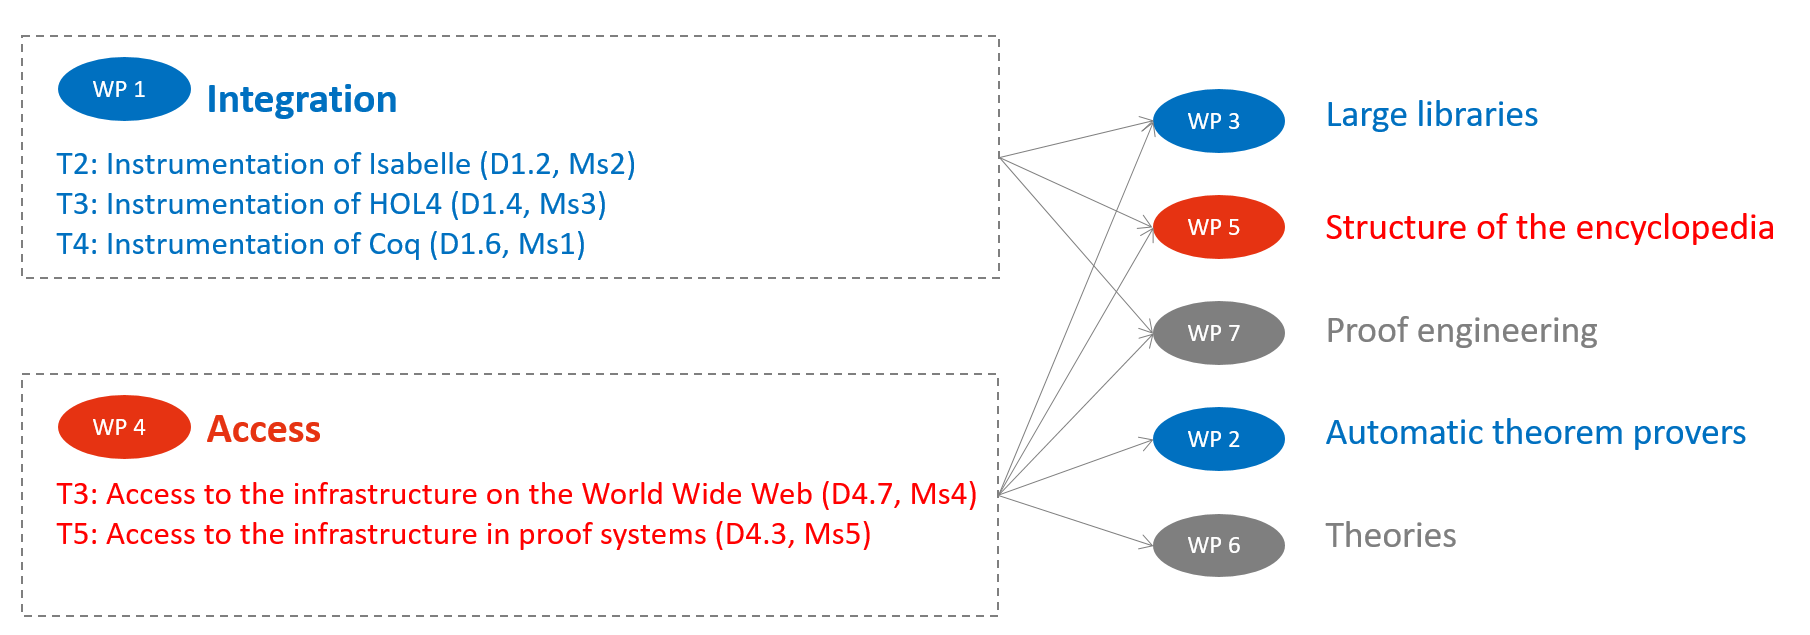
\includegraphics[width=\textwidth]{img/PERT}


%%% Local Variables:
%%%   mode: latex
%%%   mode: flyspell
%%%   ispell-local-dictionary: "english"
%%% End:


\newpage
\subsection{Work Package List}\label{sec:wplist}

\begin{todo}{from the proposal template}
Please indicate one activity per work package:
RTD = Research and technological development; DEM = Demonstration; MGT = Management of the consortium
\end{todo}

%\makeatletter\wp@total@RM{management}\makeatother
\wpfigstyle{\footnotesize}
\wpfig[pages,type,start,end]

\newpage\subsubsection*{List of all deliverables}\label{sec:deliverables}

Here is an overview of the deliverables 
of the work packages. 

%In the table below, \emph{integrating work deliverables} (see top of
%section~\ref{sec:wplist}) are printed in boldface to mark them. They integrate
%contributions from multiple work packages.

{\footnotesize\inputdelivs{8cm}}

%%% Local Variables: 
%%% mode: latex
%%% TeX-master: "propB"
%%% End: 

\newpage\subsection{List of Milestones}\label{sec:milestones}

\begin{todo}{from the proposal template}
  Milestones are control points where decisions are needed with regard to the next stage
  of the project. For example, a milestone may occur when a major result has been
  achieved, if its successful attainment is a requirement for the next phase of
  work. Another example would be a point when the consortium must decide which of several
  technologies to adopt for further development.

  Means of verification: Show how you will confirm that the milestone has been
  attained. Refer to indicators if appropriate. For examples: a laboratory prototype
  completed and running flawlessly, software released and validated by a user group, field
  survey complete and data quality validated.
\end{todo}

\ednote{maybe automate the milestones}

\ednote{Rabe: I suggest having exactly 3 milestones, namely at months 18, 36, and 48 (corresponding to the EU's review schedule), possibly more milestones in the beginning e.g., at months 6 and 12}

\begin{milestones}
  \milestone[id=kickoff,verif=Inspection,month=1]
    {Organization setup}
    {Set up the organizational infrastructure of the project: mailing lists, web site, consortium agreement, activity tracking, \ldots}

  \milestone[id=logipedia-v1,verif=Inspection,month=12]
     {Logipedia v1}
     {Release of a first version of Logipedia with HOL Light standard library and parts of Matita standard library in 5 different systems: Coq, Matita, Lean, HOL and PVS}

  \milestone[id=coq-stdlib,verif=Inspection,month=24]
     {Coq in Logipedia}
     {Integration of most of Coq standard library in Logipedia}

  \milestone[id=isabelle-stdlib,verif=Inspection,month=24]
     {Isabelle/HOL in Logipedia}
     {Integration of most of Isabelle/HOL standard library in Logipedia}

  \milestone[id=compcert,verif=Inspection,month=36]
     {CompCert in Logipedia}
     {Integration of most of the CompCert library in Logipedia}

  \milestone[id=logipedia-v2,verif=Inspection,month=36]
     {Logipedia v2}
     {Release of a second version of Logipedia integrating important parts of the libraries of Isabelle, Coq, Matita and HOL4, and their translations in other systems}

  \milestone[id=atelierb,verif=Inspection,month=48]
     {Atelier B in Logipedia}
     {Release of a tool able to translate a complete development in Atelier B into a complete Dedukti proof}

\end{milestones}

%%% Local Variables: 
%%% mode: latex
%%% TeX-master: "propB"
%%% End: 

% LocalWords:  pn ednote verif ldots


\subsection{Work Package Descriptions}\label{sec:workpackages}
\begin{workplan}
\begin{workpackage}[id=management,type=MGT,wphases=0-24!.2,
  title=Project Management,short=Management,
  FAURM=2,barRM=2,efoRM=2,bazRM=2,lead=FAU,status=canceled]
We can state the state of the art and similar things before the summary in the boxes
here. 
\wpheadertable
\begin{wpobjectives}
  \begin{itemize}
    \item To perform the administrative, scientific/technical, and financial
      management of the project
    \item To co-ordinate the contacts with the EU
    \item To control quality and timing of project results and to resolve conflicts
    \item To set up inter-project communication rules and mechanisms
  \end{itemize}
\end{wpobjectives}

\begin{wpdescription}
  Based on the Consortium Agreement, i.e. the contract with the European Commission, and
  based on the financial and administrative data agreed, the project manager will carry
  out the overall project management, including administrative management.  A project
  quality handbook will be defined, and a {\pn} help-desk for answering questions about
  the format (first project-internal, and after month 12 public) will be established. The
  project management will\ldots we can even reference deliverables:
  \delivref{management}{report2} and even the variant with a title:
  \delivtref{management}{report2}
\begin{tasklist}
  \begin{task}
    To perform the administrative, scientific/technical, and financial management of the
    project
    \end{task}
    \begin{task}
      To co-ordinate the contacts with the EU
    \end{task}
    \begin{task}
      To control quality and timing of project results and to resolve conflicts
    \end{task}
    \begin{task}[status=canceled]
      To set up inter-project communication rules and mechanisms
    \end{task}
  \end{tasklist}
\end{wpdescription}


\begin{wpdelivs}
  \begin{wpdeliv}[due=1,id=mailing,nature=O,dissem=PP,miles=kickoff,lead=FAU]
    {Project-internal mailing lists}
  \end{wpdeliv}
  \begin{wpdeliv}[due=3,id=handbook,nature=R,dissem=PU,miles=consensus,lead=FAU]
    {Project management handbook}
  \end{wpdeliv}
  \begin{wpdeliv}[due=44,id=worldpeace,nature=R,dissem=PU,status=canceled,lead=FAU]
    {Plan to save the world}
  \end{wpdeliv}
\begin{wpdeliv}[due={6,12,18,24,30,36,42,48},id=report2,nature=R,dissem=public,miles={consensus,final}]
  {Periodic activity report} 
  Partly compiled from activity reports of the work package
  coordinators; to be approved by the work package coordinators before delivery to the
  Commission.  Financial reporting is mainly done in months 18 and 36.\Ednote{how about
    these numbers?}
  \end{wpdeliv}
 \begin{wpdeliv}[due=6,id=helpdesk,dissem=PU,nature=O,miles=kickoff,lead=FAU]
    {{\pn} Helpdesk}
  \end{wpdeliv}
  \begin{wpdeliv}[due=36,id=report6,nature=R,dissem=PU,miles=final,lead=FAU]
    {Final plan for using and disseminating the knowledge}
  \end{wpdeliv}
  \begin{wpdeliv}[due=48,id=report7,nature=R,dissem=PU,miles=final,lead=FAU]
    {Final management report}
  \end{wpdeliv}
\end{wpdelivs}
\end{workpackage}

%%% Local Variables: 
%%% mode: LaTeX
%%% TeX-master: "propB"
%%% End: 

% LocalWords:  wp-management.tex workpackage efoRM bazRM wpheadertable pn ldots
% LocalWords:  wpobjectives wpdescription delivref delivtref wpdelivs wpdeliv
% LocalWords:  dissem Ednote pdataRef deliv mansubsusintReport wphases
\newpage
\begin{workpackage}%
[id=dissem,type=RTD,lead=efo,
 wphases=10-24!1,
 title=Dissemination and Exploitation,short=Dissemination,
 efoRM=8,FAURM=2,barRM=2,bazRM=2]
We can state the state of the art and similar things before the summary in the boxes
here. 
\wpheadertable

\begin{wpobjectives}
  Much of the activity of a project involves small groups of nodes in joint work. This
  work package is set up to ensure their best wide-scale integration, communication, and
  synergetic presentation of the results. Clearly identified means of dissemination of
  work-in-progress as well as final results will serve the effectiveness of work within
  the project and steadily improve the visibility and usage of the emerging semantic
  services.
\end{wpobjectives}

\begin{wpdescription}
  The work package members set up events for dissemination of the research and
  work-in-progress results for researchers (workshops and summer schools), and for
  industry (trade fairs). An in-depth evaluation will be undertaken of the response of
  test-users.

  Within two months of the start of the project, a project website will go live. This
  website will have two areas: a members' area and a public area.\ldots
\end{wpdescription}

\begin{wpdelivs}
  \begin{wpdeliv}[due=2,id=website,nature=O,dissem=PU,miles=kickoff]
     {Set-up of the Project web server}
   \end{wpdeliv}
   \begin{wpdeliv}[due=8,id=ws1proc,nature=R,dissem=PU,miles={kickoff}]
     {Proceedings of the first {\pn} Summer School.}
   \end{wpdeliv}
   \begin{wpdeliv}[due=9,id=dissem,nature=R,dissem=PP]
     {Dissemination Plan}
   \end{wpdeliv}
   \begin{wpdeliv}[due=9,id=exploitplan,nature=R,dissem=PP,miles=exploitation]
     {Scientific and Commercial Exploitation Plan}
   \end{wpdeliv}
   \begin{wpdeliv}[due=20,id=ws2proc,nature=R,dissem=PU,miles={exploitation}]
     {Proceedings of the second {\pn} Summer School.}
   \end{wpdeliv}
   \begin{wpdeliv}[due=32,id=ss1proc,nature=R,dissem=PU,miles={exploitation}]
     {Proceedings of the third {\pn} Summer School.}
   \end{wpdeliv}
   \begin{wpdeliv}[due=44,id=ws3proc,nature=R,dissem=PU,miles=exploitation]
     {Proceedings of the fourth {\pn} Summer School.}
   \end{wpdeliv}
 \end{wpdelivs}
\end{workpackage}

%%% Local Variables: 
%%% mode: LaTeX
%%% TeX-master: "propB"
%%% End: 

% LocalWords:  wp-dissem.tex workpackage dissem efo fromto bazRM wpheadertable
% LocalWords:  wpobjectives wpdescription ldots wpdelivs wpdeliv ws1proc pn
% LocalWords:  exploitplan ws2proc ss1proc ws3proc pdataRef deliv
% LocalWords:  mansubsusintReport
\newpage
\begin{workpackage}[id=class,type=RTD,lead=FAU,
                    wphases=3-9!1,
                    title=A {\LaTeX} class for EU Proposals,short=Class,
                    FAURM=12,barRM=12]
We can state the state of the art and similar things before the summary in the boxes
here. 
\wpheadertable
\begin{wpobjectives}
\LaTeX is the best document markup language, it can even be used for literate
programming~\cite{DK:LP,Lamport:ladps94,Knuth:ttb84}

  To develop a {\LaTeX} class for marking up EU Proposals
\end{wpobjectives}

\begin{wpdescription}
  We will follow strict software design principles, first comes a requirements analys,
  then \ldots
\end{wpdescription}

\begin{wpdelivs}
  \begin{wpdeliv}[due=6,id=req,nature=R,dissem=PP,miles=kickoff]
     {Requirements analysis}
   \end{wpdeliv}
   \begin{wpdeliv}[due=12,id=spec,nature=R,dissem=PU,miles=consensus]
     {{\pn} Specification }
   \end{wpdeliv}
   \begin{wpdeliv}[due=18,id=demonstrator,nature=P,dissem=PU,miles={consensus,final}]
     {First demonstrator ({\tt{article.cls}} really)}
   \end{wpdeliv}
   \begin{wpdeliv}[due=24,id=proto,nature=P,dissem=PU,miles=final]
     {First prototype}
   \end{wpdeliv}
    \begin{wpdeliv}[due=36,id=release,nature=P,dissem=PU,miles=final]
      {Final {\LaTeX} class, ready for release}
    \end{wpdeliv}
  \end{wpdelivs}
Furthermore, this work package contributes to {\pdataRef{deliv}{managementreport2}{label}} and
{\pdataRef{deliv}{managementreport7}{label}}.
\end{workpackage}

%%% Local Variables: 
%%% mode: LaTeX
%%% TeX-master: "propB"
%%% End: 
\newpage
\begin{workpackage}[id=temple,type=DEM,lead=bar,
  wphases=6-12!1,
  title={\pn} Proposal Template,short=Template,barRM=6,bazRM=6]
We can state the state of the art and similar things before the summary in the boxes
here. 
\wpheadertable

\begin{wpobjectives}
  To develop a template file for {\pn} proposals
\end{wpobjectives}

\begin{wpdescription}
  We abstract an example from existing proposals
\end{wpdescription}

\begin{wpdelivs}
  \begin{wpdeliv}[due=6,id=req,nature=R,dissem=PP,miles=kickoff,lead=bar]
    {Requirements analysis}
  \end{wpdeliv}
  \begin{wpdeliv}[due=12,id=spec,nature=R,dissem=PU,miles=consensus,lead=baz]
    {{\pn} Specification }
  \end{wpdeliv}
  \begin{wpdeliv}[due=18,id=demonstrator,nature=D,dissem=PU,miles={consensus,final},lead=bar]
    {First demonstrator ({\tt{article.cls}} really)}
  \end{wpdeliv}
  \begin{wpdeliv}[due=24,id=proto,nature=P,dissem=PU,miles=final,lead=baz]
    {First prototype}
  \end{wpdeliv}
  \begin{wpdeliv}[due=36,id=release,nature=P,dissem=PU,miles=final,lead=bar]
    {Final Template, ready for release}
  \end{wpdeliv}
\end{wpdelivs}
Furthermore, this work package contributes to {\pdataRef{deliv}{managementreport2}{label}} and
{\pdataRef{deliv}{managementreport7}{label}}.
\end{workpackage}

%%% Local Variables: 
%%% mode: LaTeX
%%% TeX-master: "propB"
%%% End: 

% LocalWords:  wp-temple.tex workpackage fromto pn bazRM wpheadertable wpdelivs
% LocalWords:  wpobjectives wpdescription wpdeliv req dissem tt article.cls
% LocalWords:  pdataRef deliv systemsintReport
\newpage
\end{workplan}
\newpage\subsection{Significant Risks and Associated Contingency Plans}\label{sec:risks}
\begin{todo}{from the proposal template}
  Describe any significant risks, and associated contingency plans
\end{todo}
\begin{oldpart}{need to integrate this somewhere. CL: I will check other proposals to see how they did it; the Guide does not really prescribe anything.}
\paragraph{Global Risk Management}
The crucial problem of \pn (and similar endeavors that offer a new basis for communication
and interaction) is that of community uptake: Unless we can convince scientists and
knowledge workers industry to use the new tools and interactions, we will
never be able to assemble the large repositories of flexiformal mathematical knowledge we
envision. We will consider uptake to be the main ongoing evaluation criterion for the network.
\end{oldpart}

%%% Local Variables: 
%%% mode: latex
%%% TeX-master: "propB"
%%% End: 



%%% Local Variables: 
%%% mode: latex
%%% TeX-master: "propB"
%%% End: 

% LocalWords:  workplan newpage wplist makeatletter makeatother wpfig
% LocalWords:  workpackages wp-dissem wp-class wp-temple
